\documentclass[12pt, a4paper, oneside]{article}
\usepackage{graphicx}
\usepackage{arial}
\renewcommand{\familydefault}{\sfdefault}
\usepackage[T1]{fontenc}
\usepackage[polish]{babel}
\usepackage[utf8]{inputenc}
\usepackage{lmodern}
\usepackage[left=2cm,right=2cm,top=2cm,bottom=2cm]{geometry}
\selectlanguage{polish}

\begin{document}
\section{Cel ćwiczenia}
\section{Spis wykorzystanych urządzeń}
\section{Przebieg ćwiczenia}
\clearpage
\section{Wyniki pomiarów}
\subsection{Linia 1}
\begin{figure}[h]
\centering
\caption{L1 k1}
\includegraphics[scale=0.28]{Linia1/k1.png}
\end{figure}
\begin{figure}[h]
\centering
\caption{L1 k2}
\includegraphics[scale=0.28]{Linia1/k2.png}
\end{figure}
\begin{figure}[h]
\centering
\caption{L1 k3}
\includegraphics[scale=0.28]{Linia1/k3.png}
\end{figure}
\begin{figure}[h]
\centering
\caption{L1 k1 stary}
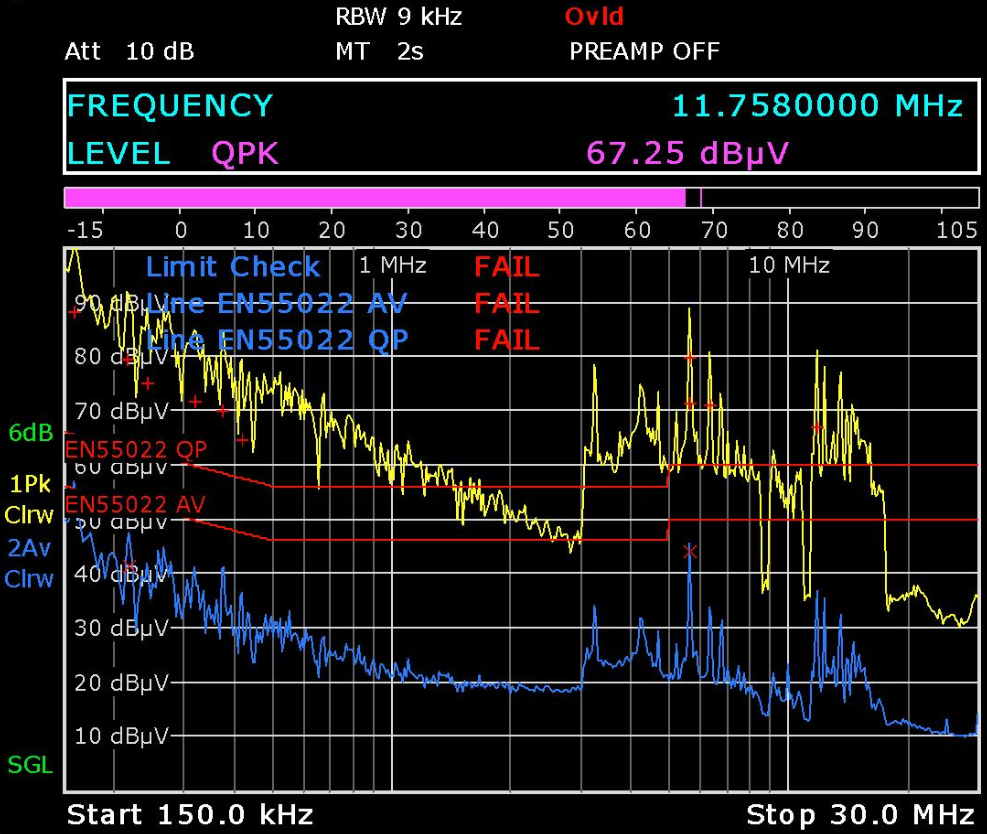
\includegraphics[scale=0.28]{Linia1/stary_k1.png}
\end{figure}
\clearpage
\subsection{Linia 2}
\begin{figure}[h]
\centering
\caption{L2 k1}
\includegraphics[scale=0.28]{Linia2/k1.png}
\end{figure}
\begin{figure}[h]
\centering
\caption{L2 k2}
\includegraphics[scale=0.28]{Linia2/k2.png}
\end{figure}
\begin{figure}[h]
\centering
\caption{L2 k3}
\includegraphics[scale=0.28]{Linia2/k3.png}
\end{figure}
\clearpage
\section{Wnioski}
\end{document}